\documentclass{article}
\usepackage{tikz}
\begin{document}

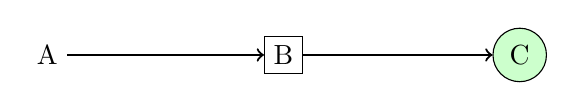
\begin{tikzpicture}[scale=1]

  % --- Plain node ---
  \node (A) at (0,0) {A};

  % --- Node with border ---
  \node[draw] (B) at (3,0) {B};

  % --- Node with border + shape + fill ---
  \node[draw, circle, fill=green!20] (C) at (6,0) {C};

  % --- Connect nodes using names ---
  \draw[->, thick] (A) -- (B);
  \draw[->, thick] (B) -- (C);

\end{tikzpicture}

\end{document}
